\scanpage{25}
\mspage{5}
des schémas $\overline{\mathrm m}$ lisses. \deleted{\unsure{i.e.}}
\diagram{\begin{tikzcd}[ampersand replacement=\&]
f:X \arrow[r,dash] \& Y.
\end{tikzcd}}

Ainsi, connaissant déjà $H^*(X^{\mathrm{an}},\mathbb C)$ comme $H_{\mathrm{DR}}^*(X)$, on aimerait une \deleted{interprétation}\inserted{construction} purement algébrique de la suite spectrale de Leray de
\diagram{\begin{tikzcd}[ampersand replacement=\&]
f^{\mathrm{an}}:X^{\mathrm{an}} \arrow[r,dash] \& Y^{\mathrm{an}}
\end{tikzcd}} :
\diagram{\begin{tikzcd}[ampersand replacement=\&]
H^*(X^{\mathrm{an}},\mathbb C) \&
E_2^{pq}=H^p(Y^{\mathrm{an}},\mathbb R^q f_*^{\mathrm{an}}(\mathbb C_{X^{\mathrm{an}}}))
\arrow[l,Rightarrow]
\end{tikzcd}}.

En fait, $\overline{\mathrm m}$ si $f$ est lisse, donc à fibres non singulières, une telle description n'est pas du tout claire en termes de ce qui a été vu jusqu'à maintenant.
\deleted{[les $\mathbb R^q f_*(\underline\Omega_{X/\mathbb C}^\bullet)$}
\inserted{Nous reviendrons sur ce point tout à l'heure.}
Un formalisme
\deleted{sont des faisceaux discrets sur $Y$, \unsure{pas des|par des}}
\figure{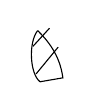
\begin{tikzpicture}[x=1cm,y=1cm]
\draw (0,0)..controls(-.12,-.15)and(-.1,-.55)..(.03,-.65);
\draw (.03,-.65)--(.32,-.6)..controls(.28,-.3)and(.12,-.12)..(0,0);
\draw (-.06,-.2)--(.15,.03);
\draw (-.02,-.55)--(.26,-.21);
\end{tikzpicture}}
\inserted{cohomologique} vraiment universel devrait impliquer, tt comme dans le cadre classique, l'écriture des suites spectrales de Leray — ce qui n'est possible que s'il englobe des ``faisceaux'' de coefficients de nature plus générale que les complexes de De Rham $\underline\Omega_X^\bullet$, — \inserted{englobant,} sans doute, également, des complexes d'opérateurs différentiels de nature plus générale que De Rham.

c) Du point de vue dualité et notions assimilées,
\margin{24}
